\documentclass[12pt, titlepage]{article}

\usepackage{booktabs}
\usepackage{tabularx}
\usepackage{hyperref}
\usepackage{float}
\usepackage{zref-xr,zref-user}

\hypersetup{
    colorlinks,
    citecolor=blue,
    filecolor=black,
    linkcolor=red,
    urlcolor=blue
}
\usepackage[round]{natbib}
\usepackage{caption}
\usepackage[letterpaper, portrait, margin=1in]{geometry}
\usepackage{helvet}
\usepackage{hyphenat}
\usepackage{pifont}

\usepackage{afterpage}
\usepackage{titlepic}
\usepackage[dvipsnames]{xcolor}
\usepackage{graphicx}

\usepackage{titlesec}
\titleformat{\section}{\large\bfseries\color{RedOrange}}{\rlap{\color{black}\rule[-0.3cm]{\linewidth}{1cm}} {\textcolor{RedOrange}{\thesection}}}{1em}{}


\renewcommand{\familydefault}{\sfdefault}
%% Comments

\usepackage{color}

\newif\ifcomments\commentstrue %displays comments
%\newif\ifcomments\commentsfalse %so that comments do not display

\ifcomments
\newcommand{\authornote}[3]{\textcolor{#1}{[#3 ---#2]}}
\newcommand{\todo}[1]{\textcolor{red}{[TODO: #1]}}
\else
\newcommand{\authornote}[3]{}
\newcommand{\todo}[1]{}
\fi

\newcommand{\wss}[1]{\authornote{blue}{SS}{#1}} 
\newcommand{\plt}[1]{\authornote{magenta}{TPLT}{#1}} %For explanation of the template
\newcommand{\an}[1]{\authornote{cyan}{Author}{#1}}

%% Common Parts

\newcommand{\progname}{ProgName} % PUT YOUR PROGRAM NAME HERE
\newcommand{\authname}{Team \#, Team Name
\\ Student 1 name and macid
\\ Student 2 name and macid
\\ Student 3 name and macid
\\ Student 4 name and macid} % AUTHOR NAMES                  

\usepackage{hyperref}
    \hypersetup{colorlinks=true, linkcolor=blue, citecolor=blue, filecolor=blue,
                urlcolor=blue, unicode=false}
    \urlstyle{same}
                                

\begin{document}

\title{\textbf{EMA Tracker for Elderly LSS Patients: System Verification and Validation Plan for \progname{}} \\ \vspace{2cm}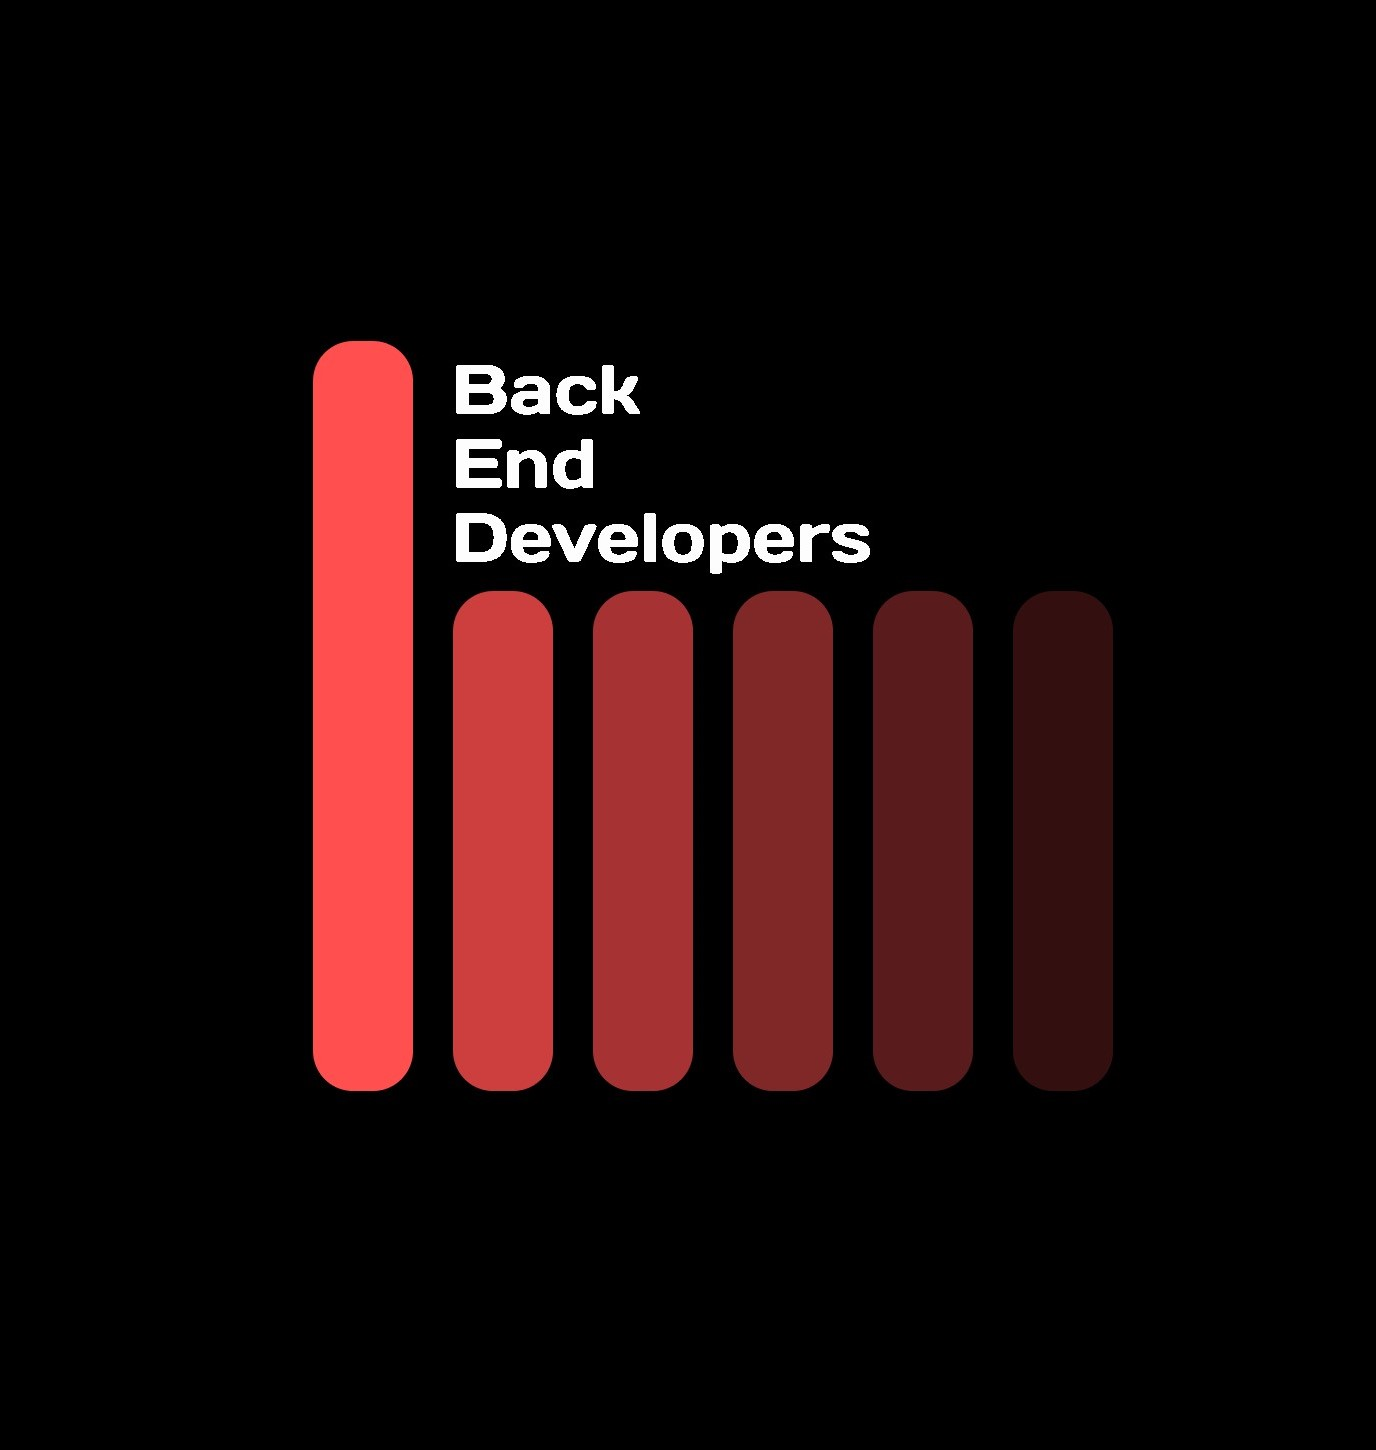
\includegraphics[width=0.5\textwidth]{../logo.jpg}}
 \pagecolor{black}\afterpage{\nopagecolor}

\author{\authname}
\date{\today}

\color{white}\maketitle
\color{black}
\pagenumbering{roman}

\section{Revision History}

\begin{tabularx}{\textwidth}{p{2.2cm}p{1.6cm}X}

  \toprule {\bf Date} & {\bf Version} & {\bf Notes}           \\
  \midrule
  2022-11-02 & 1.0 & Initial Documentation \\
  2023-03-15 & 2.0 &  Minor improvements and proof reading for revision 1 \\
  2023-03-17 & 2.1 & Incorporated TA feedback from revision 0 evaluation: Removed HST4 and added traceability for hazard analysis requirements \\
2023-04-03 & 2.2 & Added more unit testing cases \\
2023-04-04 & 2.3 & Added logo and added style to the document \\
  \bottomrule
\end{tabularx}

\newpage

\tableofcontents

\listoftables
\newpage

\section{Symbols, Abbreviations and Acronyms}
%The test plan is \href{file:../SRS/SRS}{here}.
\renewcommand{\arraystretch}{1.2}

\begin{table}[H]
	\begin{tabular}{l l} 
		  \toprule		
			  \textbf{Symbol} & \textbf{Description}\\
			  \midrule 
			  DT 						& Duration Test\\
			  MTT 					& Minor Tracking Test\\
			  PRT 					& Prompt Test\\
			  TT 						& Threshold Test\\
			  DST 					& Data Storage Test\\
			  DXT 					& Data Extraction Test\\
			  HC\#					& Hardware Constraint \#\\ 
			  SAST					& Static Application Security Testing\\			
			  DAST					& Dynamic Application Security Testing\\
			  UT						& Usability Test\\
			  PT						& Performance Test\\
			  HST					& Hardware Safety Test\\
			  RT						& Re-usability Test\\
			  DSQT					& Data Security Test\\
		  \bottomrule
	\end{tabular}\\\\
\caption{\label{Syb}Table of Symbols}
\end{table}

\newpage

\pagenumbering{arabic}

\section{General Information}

\subsection{Summary}

Researchers at the School of Rehabilitation Sciences (SReS) at McMaster University are interested in performing Ecological Momentary Assessment (EMA) for victims of spinal disorders and back pain. EMA aims to study the thoughts, experiences, and behaviours of a participant's daily life by repeatedly collecting data in an individual's normal environment, at or close to the time they carry out that behaviour.\\

The type of EMA that the SReS is interested in is focused on analyzing the daily activities and symptoms of mostly-older adults with mobility and spinal issues. They wish to track that participant's walking activity as they go about their daily life, along with prompting participants with questions when relevant events occur. The answers to event-based prompts will be combined with activity monitoring data to form a better picture about the experience this participant has with their spinal and mobility issues.\\

The EMAnator will perform EMA analysis in a manner which even older participants can use, integrated into one package which gathers relevant data about a participant's activities and allows them to easily report what is currently going on and how they feel. They also are looking for a way to access EMA data in various ways. This includes graphical representations of the data which are meaningful to researchers, along with the raw data itself. This data could be activity data, symptoms reporting data, both types of data collated together, and so on. \\

This document is intended to describe the plan for verification and validation of the device. Here, verification and validation are both technical terms with very specific meanings.\\

Verification involves checking whether or not the specifications which were described in the planning phase of the project are implemented correctly by the final system designed. Validation involves checking whether or not the product actually fulfills the needs of the end user of the device. In the words of Barry Boehm, verification asks, "Are we building the product right?" and validation asks, "Are we building the right product?"\cite{pham_1999}.

\newpage

\subsection{Objectives}

The objectives aimed to be accomplished by this verification and validation are to:

\begin{itemize}
  \item Validate if user requirements truly represent the goals of the stakeholders of the EMAnator.
  \item Validate if the input provided by the operators of the device meet the established rules and constraints.
  \item Verify if the high-level design of the device correctly fulfills the specifications of the functional and non-functional requirements.
  \item Verify if the components of the device (e.g. source code, database, physical construction, user interface, etc.) fulfill the specifications of the design.
  \item Discover any faults, failures, or malfunctions in the device.
\end{itemize}

\subsection{Relevant Documentation}

Please refer to the following documentation for reference and more information:

\begin{itemize}
  \item Development Plan: \citet{Development_Plan}
  \item Problem Statement \& Goals: \citet{Prob_n_Goals}
  \item SRS: \citet{SRS}
  \item Hazard Analysis: \citet{Hazard_Analysis}
  \item VnV Plan: \citet{VnV_Plan}
  \item Reflection: \citet{Reflection}
  \item User Guide: \citet{User_Guide}
\end{itemize}



\section{Plan}

The Verification and Validation plan will be done on both the hardware and software side individually as well as on the system integration side. The researchers, stakeholders and the Back End Developers will have different roles and techniques to test the device's functionality and usability as described below.

\pagebreak
\subsection{Verification and Validation Team}

The following table defines the different roles for the stakeholders and the Back End Developers for verification and validation.


\begin{center}
 \captionof{table}{Team roles for verification and validation.}
  \begin{tabular}{|m{5em}|m{5em}|m{25em}|}

    \hline
    \label{4_1}\textbf{Name} & \textbf{Role}                 & \textbf{Description}                                                                                                                                                                                                                                                \\
    \hline
    Dr Luciano Macedo        & End user                      & The stakeholder. She and her team of researchers will verify all the user requirements and functionality according to each sprint.                                                                                                                                                       \\
    \hline
    Jonathan Hai            & Subsystem tester              & There will be a set of test cases pre-defined for every functional requirement. Jonathan will be testing the specific functions against the test cases using unit testing, integration testing and boundary condition tests as well as SRS verification.            \\
    \hline
    Jessica Bae              & Black Box tester              & Jessica will test the specific functions of the device without knowing how the internal workflow of said device is structured. This will include stress testing for I/O for all subsytems and boundary condition testing. Valgrind will also be used for code profiling and debugging memory leaks.        \\
    \hline
    Labeeb Zaker             & Remote codebase manager       & Labeeb will ensure the codebase on GitHub has no flaws, maintain CI/CD, and review every commit added to ensure it meets the requirements without any errors.                                                                                              \\
    \hline
    Nish Shah                & Automated tester              & Nish will monitor and maintain the automated testing scripts to run certain functions against test cases that are repetitive to continuously check if the system's code functions as intended. This will be done primarily using Python code coverage tools and unit testing frameworks for code development (unittest, Coverage.py). \\
    \hline
    Anish Rangarajan         & Hardware \& Automated tester  & Anish will verify and test embedded hardware designs in C using Cunit and bullseye coverage for unit testing framework and code coverage.                                                                                                                      \\
    \hline
    Oliver Foote             & White Box \& Database testing & Oliver will test the internal workflow for valid outputs. Database validation will be performed using Orion for stress testing of I/O and database functionality.                                                                               \\
    \hline
  \end{tabular}

\end{center}

\pagebreak
\subsection{SRS Verification Plan}\label{SRS_verification}

The SRS will be verified according to a checklist. It will also follow a rigorous task based inspection listed in the table below. This is to make sure all the requirements and goals receive several iterations of verification and validation.


\begin{center}
\captionof{table}{SRS verification checklist and task based inspection}
  \begin{tabular}{|m{2cm}|m{9cm}|m{4cm}|}
    \hline
    \textbf{Section }                                 & \textbf{Description}                                                                                                                                                                  & \textbf{Approach \newline of Feedback}
    \\
    \hline
    Overall                        & The verification will be done based on an ad hoc approach through the checklist below: \begin{itemize}
                                                                                                                                                       \item[\ding{111}] System constrains for hardware and software are valid.
                                                                                                                                                       \item[\ding{111}] Monitored and controlled variables are consistent.
                                                                                                                                                       \item[\ding{111}] Comparison to existing solutions is unambiguous.
                                                                                                                                                       \item[\ding{111}] Project Goals are relevant to description of device.
                                                                                                                                                     \end{itemize}                                                                                & Will be done by Stakeholder Dr. Luciana Macedo, supervisor, classmates and the Back End Developers. \\
    \hline
   4.1-4.3                      & The verification for this section will be performed by checking if system constrains and user characteristics are provided in detail without any ambiguity.                                       & Will be done by team member Jonathan Hai.                                                    \\
    \hline
    5                  &  Terminology and the use of monitored and controlled variables must be verified to be consistent and correct. Assumptions are clearly mentioned and provided along with goals of the project. & Will be done by team member  Nish Shah.                                                      \\
    \hline
  7                     & Functional and non-functional requirements must be verified. In addition, the requirements must be checked to see if they are classified correctly. Checking required behaviour as well.                              & Will be done by team member Anish Rangarajan.                                                \\
    \hline
8-12&  Matrices and graphs must be verified according to requirements. In addition, verification must be performed to see if normal operation covers the required goals of the device.                                         & Will be done by team member Labeeb Zaker.                                                    \\
    \hline
14-16                                           & The FSM, Legal factors and Phase in Plan must be verified.                                                                                                                                 & Will be done by team member Jessica Bae.                                                     \\
    \hline
  \end{tabular}
\end{center}
\pagebreak

%%%%%%%%%%%%%%%%%%%%%%%%%%%%%%%%%%%%%%%%%%%%%%%%%%%%%%%%%%%%%%%%%%%%%%%%%%%%%%%%%%%%%%%%%%%%%%
\subsection{Design Verification Plan}
\captionof{table}{Plan for verification of the design of the system.}
\begin{tabular}{|p{4cm}|p{8cm}|p{4cm}|}
  \hline
  \label{sec_4_3}\textbf{Test Categories} & \textbf{Description}                                                                                                                                                                                                                                                                                                 & \textbf{Approach}                      \\
  \hline
  Response Feedback Test                  & This test will test the majority of the sensors of the system. Sensor input will be pushed beyond the established boundaries in different testing scenarios, with feedback being observed for erraneous or strange readings.
 & Performed by \newline Anish Rangarajan and stakeholders\\
  \hline
  User Interface Test                     & Different elements of the user interface will tested by manipulating said elements in all possible scenarios. In addition, characteristics such as screen size, brightness, and visibility will be tested in different visual environments to determine whether or not they are visible in the correct ranges of use.                                                                                                              & Performed by \newline Nish Shah                \\
  \hline
  Durability Test                         & Each sensor will be tested for failure independence. Should one sensor fail, it must not impact the functionality of any other sensors of the system. To test this, individual sensors will be rendered non-functional, and other sensor values will be checked for erroneous readings.                                                                         & Performed by Jonathan Hai                \\
  \hline
  Database Scalability Test               & This system's database will be tested for volume overload issues. Postman (a request tool) will be used to feed as many requests as possible to the database. The database will then be monitored for faults and errors. & Performed by \newline Labeeb Zaker                \\
  \hline
  Hardware \newline Communication Test                & Valgrind will be used at every interaction between hardware components to determine whether or not memory has been allocated properly. An execution tracker will also be used to ensure the workflow is functioning as expected.                                                                                                          & Performed by \newline Jessica Bae                \\
  \hline
\end{tabular}

\pagebreak
\subsection{Verification and Validation Plan Verification Plan}

Since the VnV plan is focused on validating the functionalities of the device through verification of different test cases, the only way to verify this document is to check for all such scenarios and their expected results.\\
\\The following will be done to verify the VnV plan:\\
\begin{itemize}
  \item[\ding{111}] Each task will be verified as per \hyperref[4_1]{4.1} throughout the development phase. Verifiers must ensure that tests do not fail at any of the expected scenarios and works as expected from user's point of view.
  \item[\ding{111}] Each section of the SRS will be verified as per \hyperref[SRS_verification]{4.2}. Each variable needs to be controlled accordingly and specific scenarios need to be tested to ensure functionality without errors.
  \item[\ding{111}] Each component of the design must be verified as per \hyperref[sec_4_3]{4.3} as it is being developed, so that unit testing can be performed and evaluated before system testing.
  \item[\ding{111}] Code-review meetings must be attended by all code evaluators. If an evaluator fails to join the review, the review will be rescheduled. Tests will be performed against all possible scenarios to ensure all cases work as intended.
  \item[\ding{111}] All test cases for each functional requirement as per \hyperref[sec_5_1]{5.1} must be verified accordingly by ensuring that the outputs are expected and within bounds, and that variables are being properly controlled and monitored.
\end{itemize}

%%%%%%%%%%%%%%%%%%%%%%%%%%%%%%%%%%%%%%%%%%%%%%%%%%%%%%%%%%%%%%%%%%%%%%%%%%%%%%%%%%%%%%%%%%%%%%
\subsection{Implementation Verification Plan}

The Implementation Verification Plan will utilize static and dynamic code analysis as the debugging methods to find bugs early in development. The checklist below can be used in development to follow the implementation verification plan.\\
The following methods will be used for static code analysis:
\begin{itemize}
  \item Bi-weekly code review with sub-teams (hardware, software, frontend/backend) for code walk through.
  \item Weekly code review with entire team for system-level software design.
  \item A SAST tool will be used to scan source code, binary and byte code to reveal vulnerabilities.
  \item Static analysis tools such as Pylint and lint described in \ref{Automation} will be used to find bugs in code.
\end{itemize}
Dynamic code testing will help identify exploitable vulnerabilities. The following methods will be used for dynamic code analysis:
\begin{itemize}
  \item A DAST tool will be used as a black-box tester. It will input malicious SQL queries, long input strings and invalid data to exploit assumptions made by the developers.
  \item Modular code will  be run separately against a variety of inputs to find bugs in code.
  \item Open source tools will be used based on the programming language (CrossHair for Python, CHAP for C) to provide a comprehensive view of performance and security of the device.
\end{itemize}


\subsection{Automated Testing and Verification Tools}\label{Automation}

Automated testing and verification tools will be selected based on the different programming languages and tools used in the development of the device. As covered in the development plan \cite{Development_Plan} the following unit testing frameworks, profiling tools and linters will be used for verification of code:

\begin{itemize}
  \item Python:
        \begin{itemize}
          \item unittest will be used as the Unit testing framework for Python to cover test automation, aggregation of tests (integration 							testing) and independence of tests from the reporting framework.
          \item Coverage.py will be used to measure code coverage and to gauge the effectiveness of tests performed.
          \item Pylint will be used as the linter/static code analyser which will check for errors and enforce a coding standard.
        \end{itemize}
  \item C:
        \begin{itemize}
          \item CUnit will be used as a unit testing framework for embedded system development.
          \item Bullseye coverage will be used for C code coverage analysis.
          \item lint will be used as the linter/static code analyser for development in C.
        \end{itemize}
  \item Valgrind will be used for Python (pytest-valgrind) and C as a debugging tool for code profiling.
  \item Orion will be used for SQL/Database testing. It will be used to stress test I/O coverage and to make sure the database functions as expected.
\end{itemize}

\subsection{Software Validation Plan}

There will be no plan for Software validation since there is no external data used and all the software-related validations are covered in  section \ref{SRS_verification}.

\section{System Test Description}

\subsection{Tests for Functional Requirements}\label{sec_5_1}

%%%%%%%%%%%%%%%%%%%%%%%%%%%%%%%%%%%%%%%%%%%%%%%%%%%%%%%%%%%%%%%%%%%%%%%%%%%%%%%%%%%%%%%%%%%%%%%%%%%%%%%%
\subsubsection{Duration Test}

The following tests will check whether the device will maintain an "ON" state throughout the duration of the monitoring period. The primary tests will involve different monitoring periods with valid inputs, invalid inputs, past dates, or dates too far into the future beyond what the battery life can sustain (HC2).
		
\begin{enumerate}

	\item{\textbf{DT\_1: Regular Inputs}\\}\label{DT1}
		
		Control: Manual, Dynamic
							
		Initial State: Device waits for the monitoring period to be set up in the configuration of the device.
							
		Input: Monitoring Period ["Date","Time"]  : ["03-11-2022", "05:30:PM"].
		
		Output: Device turns off after monitoring period.
							
		How test will be performed: The test is performed by passing in a valid monitoring period and ensuring that the device maintains power throughout this period.
					
	\item{\textbf{DT\_2: Invalid Inputs}\\}\label{DT2}
	
		Control: Manual, Dynamic
							
		Initial State: Device waits for the monitoring period to be set up in the configuration of the device.
							
		Input: Monitoring period ["Date","Time"] : ["3rd November 2022", "Five Thirty PM"].
							
		Output: Device returns an error code to the error handler and asserts the Invalid Data Error (BED\_ERR\_INVALID\_DATA).
		
		How test will be performed: The test is performed by passing an invalid input and ensuring the appropriate error code is returned.

\newpage
	\item{\textbf{DT\_3: Earlier Date}\\}\label{DT3}
		
		Control: Manual, Dynamic
							
		Initial State: Device waits for the monitoring period to be set up in the configuration of the device.
							
		Input: Monitoring period ["Date","Time"] : ["01-1-1999", "05:30:PM"].
							
		Output: Device returns an error code to the error handler and asserts the Invalid Data Error (BED\_ERR\_INVALID\_DATA).
		
		How test will be performed: The test is performed by passing an old date (prior to current date).

	\item{\textbf{DT\_4: Date Beyond Capabilities}\\}\label{DT4}
		
		Control: Manual, Dynamic
							
		Initial State: Device waits for the monitoring period to be set up in the configuration of the device.
							
		Input: Monitoring period ["Date","Time"] : ["9-12-2300", "05:30:PM"].
							
		Output: Device returns an error code to the error handler and asserts the Invalid Data Error (BED\_ERR\_INVALID\_DATA).

		How test will be performed: The test is performed by passing a date greater than what the battery life of the device can support.

\end{enumerate}
%%%%%%%%%%%%%%%%%%%%%%%%%%%%%%%%%%%%%%%%%%%%%%%%%%%%%%%%%%%%%%%%%%%%%%%%%%%%%%%%%%%%%%%%%%%%%%%%%%%%%%%%

\subsubsection{Device should track Minor Movements}
The following tests will be run to ensure that the device is able to track activities to a resolution deemed sufficient for general activity tracking. Tests will involve varying the rate at which the device is moved, rotated, oriented, etc. and checking if the status of the sensors is valid.

\paragraph{Minor Tracking Test}
\begin{enumerate}
	\item{\textbf{MTT\_1: Regular Movement} \\}\label{MTT1}
	
		Control: Manual, Dynamic
							
		Initial State: Device is worn with all systems working.
							
		Input: Tester performs activities at a regular/normal pace.
		
		Output: Status returned by the sensor array is no error (BED\_ERR\_NONE) and no prompt should be generated (stay in idle-mode).

		How test will be performed: The test is performed by strapping the device onto a tester who will perform the tracked activities between 60 - 100 BPM heartrate and walking pace, the tester should not have to feel any level of excessive effort for this level of activity. This is done to ensure that the device is functional under "normal" scenarios and is able to differentiate it from "no activity". If tester's heart rate is not within the specified limit, the particular set of data is to be disregarded.

	\item{\textbf{MTT\_2: Slow Movement} \\}\label{MTT2}
	
		Control: Manual, Dynamic
							
		Initial State: Device is worn with all systems working.
							
		Input: Tester performs activities at a very slow pace.
		
		Output: Status returned by the sensor array is no error (BED\_ERR\_NONE) and all sensor data are correctly stored within microSD.
		
		How test will be performed: The test is performed by strapping the device onto a tester who will walk at a speed that would exceed 12 steps per 1 minute. Then microSD is inserted into a PC to examine its contents. This is done to ensure that the device can recognize and differentiate slow movements from regular paced movements and capture corresponding sensor data.\\


\end{enumerate}
%%%%%%%%%%%%%%%%%%%%%%%%%%%%%%%%%%%%%%%%%%%%%%%%%%%%%%%%%%%%%%%%%%%%%%%%%%%%%%%%%%%%%%%%%%%%%%%%%%%%%%%%
\subsubsection{Prompt Tests}

The following tests will be done to ensure that the proper information is prompted to the user when activities are detected. Tests involve generating the test prompt, and generating prompts for different activities.

\begin{enumerate}
	\item{\textbf{PRT\_1: Test Prompt} \\}\label{PRT1}
	
		Control: Manual, Dynamic
							
		Initial State: Device has just been reconfigured.
							
		Input: Device is powered on.
		
		Output: Test Prompt is displayed.

		How test will be performed: The test is performed by turning on the device for the first time after reconfiguration. Upon turning on the device, tester should receive a test prompt that to confirm that the prompting system is working correctly. This prompt should not be dependent of any user activities.\\\\
		Test Prompt: Is this Device on?\\
		Possible Answers: Yes or No
		
	\item{\textbf{PRT\_2: Activity Prompt} \\}\label{PRT2}
	
		Control: Manual, Dynamic
							
		Initial State: Device is in the idle state.
							
		Input: Walk for 5 seconds and then limp for 5 seconds.
		
		Output: Prompt is generated to ask a question to the tester.
							
		How test will be performed: The test is done by having a tester imitate limping activity. The walking portion of the activity should be performed under the same critera as MTT\_1.\\\\
		Prompt: Are you in pain?\\
		Response choices: Yes, No
\end{enumerate}

\subsubsection{Customizable Thresholds}

The following tests will be done to ensure that the proper information is prompted to the user when activities are detected. Tests involve generating the test prompt, and generating prompts for different activities.
		
\begin{enumerate}
	\item{\textbf{TT\_1: Regular Inputs} \\}\label{TT1}
	
		Control: Manual, Dynamic
							
		Initial State: Device is in Configuration mode.
							
		Input: Regular values for thresholds within limits.
		
		Output: Config File generated successfully.
		
		How test will be performed: The test is performed by setting the device to configuration mode and then setting valid values for the thresholds.\\
		eg: \\
		Speed Threshold:\\
		Limits: 0m/s \textless Threshold \textless 5m/s

	\item{\textbf{TT\_2: Below Lower Limit} \\}\label{TT2}
	
		Control: Manual, Dynamic
							
		Initial State: Device is in Configuration mode.
							
		Input: Values for thresholds below lower limits.
		
		Output: Config File generates a BED\_ERR\_OUT\_OF\_BOUNDS.

		How test will be performed: The test is performed by setting the device to configuration mode and then setting values for the thresholds above allowable limits.

\pagebreak

	\item{\textbf{TT\_3: Above Upper limit }\\}\label{TT3}
	
		Control: Manual, Dynamic
							
		Initial State: Device is in Configuration mode.
							
		Input: Values for thresholds above upper limits.
		
		Output: Config File generates a BED\_ERR\_OUT\_OF\_BOUNDS.
		
		How test will be performed: The test is performed by setting the device to configuration mode and then setting values for the thresholds below allowable limits.

	\item{\textbf{TT\_4: Invalid Value} \\}\label{TT4}
	
		Control: Manual, Dynamic
							
		Initial State: Device is in Configuration mode.
							
		Input: Invalid values for thresholds.
		
		Output: Config File generates a BED\_ERR\_INVALID\_DATA.
		
		How test will be performed: The test is performed by setting the device to configuration mode and then setting invalid values for the thresholds.

	\item{\textbf{TT\_5: No Value} \\}\label{TT5}
	
		Control: Manual, Dynamic
							
		Initial State: Device is in Configuration mode.
							
		Input: No values for thresholds.
		
		Output: Config File generates a BED\_ERR\_INVALID\_DATA.

		How test will be performed: The test is performed by setting the device to configuration mode and then setting no values for the thresholds.
\end{enumerate}
%%%%%%%%%%%%%%%%%%%%%%%%%%%%%%%%%%%%%%%%%%%%%%%%%%%%%%%%%%%%%%%%%%%%%%%%%%%%%%%%%%%%%%%%%%%%%%%%%%%%%%%%
\pagebreak
\subsubsection{Data Storage}

The following tests will be done to ensure that data is stored when appropriate. Tests include checking when storage buffer is full, when prompts are generated and when sensor data needs to be logged. 
\begin{enumerate}
	\item{\textbf{DST\_1: Storage Buffer Full} \\}\label{DST1}
	
		Control: Manual, Dynamic
							
		Initial State: Device is in an idle state.
							
		Input: Activity detected causing prompt to be generated (Internal storage is full).
		
		Output: Data Storage system generates a BED\_ERR\_MEMORY\_FULL
		
		How test will be performed: The test is performed by first loading the internal memory buffer with garbage values so that it is nearly/completely full. Then a registered activity is triggered generating a 					prompt. Once this is answered, the system will not have enough memory to store the new values thus resulting in an error.

	\item{\textbf{DST\_2: Prompt Generated} \\}\label{DST2}
	
		Control: Manual, Dynamic
							
		Initial State: Device is in an idle state.
							
		Input: Activity detected causing prompt to be generated.
		
		Output: Prompt Response is saved into the internal memory.
		
		How test will be performed: The test performs registered activities and ensuring that the prompt generated is answered and its result is stored in the internal storage buffer.\\
		eg: Registered Activity: Participant slows down or comes to a stop for an extended period of time\\
		Prompt Generated: \\
		Are you in pain?\\
		Possible Answers: Yes or No\\
		\\
		Prompt Generated: \\
		Do you need assistance?\\
		Possible Answers: Yes or No\\
\pagebreak
	\item{\textbf{DST\_3: Sensor Storage} \\}\label{DST3}
	
		Control: Manual, Dynamic
							
		Initial State: Device is in an idle state.
							
		Input: Activity detected causing prompt to be generated.
		
		Output: Specific sensor values that triggered a prompt are stored in the internal memory.
							
		How test will be performed: The test performs registered activities and ensuring that the sensor values that caused the prompt are stored in the internal storage buffer.
\end{enumerate}
%%%%%%%%%%%%%%%%%%%%%%%%%%%%%%%%%%%%%%%%%%%%%%%%%%%%%%%%%%%%%%%%%%%%%%%%%%%%%%%%%%%%%%%%%%%%%%%%%%%%%%%%
\subsubsection{Data Extraction}

The following tests will be done to ensure that data can be extracted and presented in a graphical manner deemed acceptable for the purpose of EMA analysis.
\begin{enumerate}
	\item{\textbf{DXT\_1: Extracting Data} \\}\label{DXT1}
	
		Control: Manual, Dynamic
							
		Initial State: Device is connected to the device manager.
							
		Input: A command that tells the device manager to extract all data from the internal memory.
		
		Output: Extracted data is sent to the Host Software where it is converted to a presentable form.

		How test will be performed: The test is performed by first running the device as intended and waiting for a small monitoring period to finish. After this the device is connected to the host software with the 				help of the device manager driver. Once connected, the user can start the extraction process and should be able to see all the relevant data in a presentable manner.
		
	\item{\textbf{DXT\_2: Extracting No Data} \\}\label{DXT2}
	
		Control: Manual, Dynamic
							
		Initial State: Device is connected to the device manager.
							
		Input: A command that tells the device manager to extract all data from the internal memory.
		
		Output: Device Manager returns a BED\_ERR\_EMPTY\_DATA error

		How test will be performed: The test is performed by first deleting all the contents of the internal memory prior to connection with the host software. Once connected and the extraction process begins, the 				system should return an error due to no data being present to extract.

	\item{\textbf{DXT\_3: Extracting Corrupted Data} \\}\label{DXT3}
	
		Control: Manual, Dynamic
							
		Initial State: Device is connected to the device manager.
							
		Input: A command that tells the device manager to extract all data from the internal memory.
		
		Output: Device Manager returns a BED\_ERR\_INVALID\_DATA error

		How test will be performed: The test is performed by first deleting all the contents of the internal memory and filling it with garbage values prior to connection with the host software. Once connected and 				the extraction process begins, the system should return an error due to corrupted data being present to extract.
\end{enumerate}
%%%%%%%%%%%%%%%%%%%%%%%%%%%%%%%%%%%%%%%%%%%%%%%%%%%%%%%%%%%%%%%%%%%%%%%%%%%%%%%%%%%%%%%%%%%%%%%%%%%%%%%%
\subsection{Tests for Nonfunctional Requirements}
\subsubsection{Hardware Safety }

These tests are designed to test the safety of the device concerning electrical and hardware components. It is important that the users of the device are kept safe, that any systems in place to protect them from electrical shocks are functioning properly, and that the indicator LED functions as expected under certain conditions.

\begin{enumerate}

\item{\textbf{HST\_1: High Voltage}}\label{HST1}

Control: Manual, Dynamic

Initial State: Device begins in "off" mode.

Input: When the device is turned on a voltage over expected voltage is applied.

Output: Device detects high voltage and indicates that voltage is high using an indicator LED. The breaker or fuse then trips or the voltage is sent to ground.

Test Case Derivation: N/A

How test will be performed: Use a power supply to oversupply the system with voltage. 

\item{\textbf{HST\_2: Normal Voltage}}\label{HST2}

Control: Manual, Dynamic

Initial State: Device begins in "off" mode.

Input: When device is turned on a normal voltage is applied.

Output: Device powers on, no issues are detected.

Test Case Derivation: N/A

How test will be performed: The power supply will be used to provide the expected voltage to the device.

\item{\textbf{HST\_3: Low Voltage}}\label{HST3}

Control: Manual, Dynamic

Initial State: Device begins in "off" mode.

Input: When device is turned on a voltage below the expected amount is applied.

Output: If device powers on, indicator LED indicates that the voltage is lower than expected, device goes into power saving mode.

Test Case Derivation:

How test will be performed: Use power supply to provide a lower than expected voltage to the device.

\end{enumerate}

\subsubsection{Reusability}

These tests will evaluate the re-usability of various hardware systems of the device. The device should be reusable by multiple participants to prevent electronic waste and reduce cost for the researchers. 

\begin{enumerate}

%add another test or gear test toward charge protection, circuitry to stop overcharging/discharging.

\item{\textbf{RT\_1: Battery Charge/Discharge}}\label{RT1}

Control: Manual, Dynamic

Initial State: Battery is fully discharged.

Input: Connect battery to the charging cable.

Output: Battery is fully charged without issue.

Test Case Derivation: N/A

How test will be performed: Battery component will be isolated from device and fully charged and discharged 5 times.

\item{\textbf{RT\_2: Battery Charge Protection}}\label{RT2}

Control: Manual, Dynamic

Initial State: Battery is fully charged.

Input: Connect battery to the charging cable.

Output: Battery will not overcharge.

Test Case Derivation: N/A

How test will be performed: Battery component will be isolated from device and fully charged. The battery will then plugged in to the charger for 5 minutes.

\end{enumerate}

\subsubsection{Accuracy}
The following set of tests will ensure that the device can recognize its state and perform its main functionality in accurate manner.
The following functional requirements test cases are applicable for accuracy:

\begin{itemize}
\item MTT\_1: \hyperref[MTT1]{Regular Movement}
\item MTT\_2: \hyperref[MTT2]{Slow Movement}
\item PRT\_1: \hyperref[PRT1]{Test Prompt}
\item PRT\_2: \hyperref[PRT2]{Activity Prompt}
\end{itemize}

\subsubsection{Usability}
The following set of tests will ensure that the device is usable by target user population and cause no problems in terms of maintenance and user interactions.		
\begin{enumerate}

\item\textbf{{UT\_1: Device UI\\}}\label{UT1}

Type: Manual, Static
					
Initial State: The device is turned on and a question prompt is generated on screen.
					
Input/Condition: Testers are asked to answer the questionnaire set without assistance in less than 1 minute.
					
Output/Result: All testers are able to answer their prompt successfully.
					
How test will be performed: A test group of people with age of 40 or older will be asked to receive a powered-on EMAnator and asked to respond to a set of 3 questions in 1 minute. These questions will randomly be selected from the following 10 questions.

\begin{itemize}
\item Are you a dog person or a cat person?
\item Are you currently inside of a building?
\item Are you currently a student?
\item Did you make your bed this morning?
\item Do you feel tired right now?
\item Do you prefer coffee or tea?
\item Do you have a G driver's license?
\item Do you feel sleepy right now?
\item Which is better: Summer vs Winter
\item Is it daytime right now?
\end{itemize}
					
\item\textbf{{UT\_2: Comfortable Device\\}}\label{UT2}

Type: Manual, Static
					
Initial State: The device is turned on and left on idle mode.
					
Input: Testers are asked to wear the device for 24 hours.
					
Output: Testers fill out a survey form regarding the comfort of the device on their body.
					
How test will be performed: At the end of their 1 day cycle, testers will be asked to fill out an online form indicating how comfortable they felt the device was regards to weight, shape, stability, etc. The following questions will be asked.

\begin{itemize}
\item Did the device every fall off? If so, please record the following for each case: What you were doing each time? When did the incident happen?
\item How do you feel regarding the weight of the device? Was it too heavy or too light?
\item How do you feel regarding the texture of the device? Did you find it uncomfortable in any way?
\end{itemize}

\item\textbf{{UT\_3: Reusability\\}}\label{UT3}

Type: Manual, Static
					
Initial State: The device is cleaned using isopropyl alcohol wipes.
					
Input: Testers visually inspect how clean the device is.
					
Output: The device is deemed clean and the device is not harmed.
					
How test will be performed: 1 member of Back End Developers will clean the device and 5 other members will inspect and judge if the device is clean enough to be reused. Among the 5 inspecting members, 1 member will then turn on the device to make sure that there was no harm done to the device while cleaning it.

\item\textbf{{UT\_4: Host Software UI\\}}\label{UT4}

Type: Manual, Static
					
Initial State: Main page displayed after login page.
					
Input: Testers try to filter out database record of anyone 70 years old and write down the first names.
					
Output: John, Marry, Bill
					
How test will be performed: The software application is presented with its main page. Testers are required to navigate through the software to use the dataview filtering functionality and filter out data as requested by the test. They are then asked to write down their responses on a piece of paper. Later, the papers are collected and compared for validation.

\end{enumerate}


\pagebreak
\subsubsection{Performance}
The following set of questions will ensure that the device is capable of meeting user expectations.
\begin{enumerate}
\item\textbf{{PT\_1: Data Transfer Time\\}}\label{PT1}

Type: Automatic, Dynamic
					
Initial State: The device has collected a complete set of data.
					
Input: The device is connected to the host software and connection is established for data transfer.
					
Output: Data transfer to finish within the specified parameter, TRASFER\_TIME.
					
How test will be performed: 2 group members of the Back End Developers will each perform data transfer tests 3 times and record the total transfer time for each execution. All 6 tests should result in execution time less than or equal to TRANSFER\_TIME.

\item\textbf{{PT\_2: Battery Life\\}}\label{PT2}

Type: Automatic, Static
					
Initial State: The device is turned on and left on idle mode.
					
Input: Testers wear the device for standard monitoring period.
					
Output: The total amount of time before the device runs out of battery is greater or equal to the parameter, BATTERY\_LIFE.
					
How test will be performed: 2 group members of the Back End Developers each wear the device for standard monitoring period under their normal lives. At the end of each calendar day, they are asked to record their response to a simple question: "Does the device still have battery life left? If so, how much percentage?". 

\end{enumerate}
\pagebreak
\subsubsection{Data Security Tests}

These tests are designed to test the security of the system and the accessibility of important medical records. Ensuring that only certain people are able to access these records is a vital part of the design, and ensuring that records cannot be modified is also important for research data integrity. 

\begin{enumerate}

\item{\textbf{DSQT\_1: Records Safety Test}}\label{DSQT1}

Control: Manual, Dynamic

Initial State: Device is powered on.

Input: Data transfer cable is plugged in from device to a generic PC, a tester tries to access the database and modify the data within.

Output: Database inaccessible and requests an administrative security key. The tester should be unable to access or modify the data.

Test Case Derivation: N/A

How test will be performed: Device will be given to a tester with technical know-how who does not have access to the administrator security key. They will attempt to access the database. 

\item{\textbf{DSQT\_2: Data Storage Selection Test}}\label{DSQT2}

Control: Manual, Dynamic

Initial State: Device is powered on.

Input: Less than 3 seconds of limping from tester.

Output: Corresponding sensor data is not included in sdcard data.

Test Case Derivation: N/A

How test will be performed: One member of Back End Developers wears the device and pretends to "limp" for 3 seconds, to create garbage sensor data. Then microSD card is inserted in to a PC to examine the content. 

\end{enumerate}



\subsection{Traceability Between Test Cases and Requirements}

%Traceability Matrix, needs lot of updating, it also doesn't function rn...

\noindent
\begin{table}[H]
	\centering
	\begin{tabular}{|c|c|c|c|c|c|c|c|c|c|}
	\hline
		& \hyperref[DT1]{DT1}& \hyperref[DT2]{DT2}&\hyperref[DT3]{DT3}& \hyperref[DT4]{DT4} &\hyperref[MTT1]{MTT1}&\hyperref[MTT2]{MTT2}&\hyperref[PRT1]{PRT1}&\hyperref[PRT2]{PRT2}&\hyperref[TT1]{TT1} \\
	\hline       
	\textbf{R1}         &X&X&X&X&&&&& \\ \hline
	\textbf{R2}         &&&&&X&X&&&\\ \hline
	\textbf{R3}         &&&&&&&X&X& \\ \hline
	\textbf{R4}         &&&&&&&&&X\\ \hline
	\textbf{R5}         &&&&&&&&& \\ \hline
	\textbf{R6}         &&&&&&&&&\\ \hline
	\textbf{NFR1}     &&&&&X&X&X&X& \\ \hline
	\textbf{NFR12}   &&&&&&&X&&\\ \hline
	\hline
	\end{tabular}
	\caption{ Requirements Traceability Matrix Part 1}
	\label{Table:A_trace}
\end{table}



\begin{table}[H]
	\centering
	\begin{tabular}{|c|c|c|c|c|c|c|c|c|c|c|}
	\hline
	& \hyperref[TT2]{TT2}&\hyperref[TT3]{TT3}& \hyperref[TT4]{TT4} &\hyperref[TT5]{TT5}&\hyperref[DST1]{DST1}&\hyperref[DST2]{DST2}&\hyperref[DST3]{DST3}&\hyperref[DXT1]{DXT1}&\hyperref[DXT2]{DXT2}&\hyperref[DXT3]{DXT3} \\
	\hline     
	\textbf{R1}         &&&&&&&&&& \\ \hline
	\textbf{R2}       	 &&&&&&&&&&\\ \hline
	\textbf{R3}         &&&&&&&&&& \\ \hline
	\textbf{R4}         &X&X&X&X&&&&&&\\ \hline
	\textbf{R5}          &&&&&X&X&X&&& \\ \hline
	\textbf{R6}         &&&&&&&&X&X&X\\ \hline
	\hline
	\end{tabular}
	\caption{Requirements Traceability Matrix Part 2}
	\label{Table:B_trace}
\end{table}

\begin{table}[H]
	\centering
	\begin{tabular}{|c|c|c|c|c|c|c|c|c|c|c|c|c|}
	\hline
	& \hyperref[HST1]{HST1}&\hyperref[HST2]{HST2}& \hyperref[HST3]{HST3}&\hyperref[RT1]{RT1}&\hyperref[RT2]{RT2}&\hyperref[UT1]{UT1}&\hyperref[UT2]{UT2}&\hyperref[UT3]{UT3}&\hyperref[UT4]{UT4}&\hyperref[PT1]{PT1}&\hyperref[PT2]{PT2}&\hyperref[DSQT1]{DSQT1} \\
	\hline       
	\textbf{NFR2}         &&&&&&X&X&X&X&&&\\ \hline
	\textbf{NFR3}         &&&&&&&&&&&X& \\ \hline
	\textbf{NFR4}         &&&&&&&X&&&&&\\ \hline
	\textbf{NFR5}         &&&&&&&&X&&&& \\ \hline
	\textbf{NFR6}         &X&X&X&&&&&&&&&\\ \hline
	\textbf{NFR7}         &&&&X&&&&&&&&\\ \hline
	\textbf{NFR8}         &&&&&&&&&&&&X\\ \hline
	\textbf{NFR9}         &&&&&&X&&&X&&&\\ \hline
	\textbf{NFR10}       &&&&&&X&&&X&&&\\ \hline
	\textbf{NFR11}       &X&X&X&X&&&&&&&&\\ \hline
	\textbf{NFR13}       &&&&&&&&&&X&&\\ \hline
	\textbf{NFR14}       &&&&&&&&&&&&X\\ \hline
	\hline
	\end{tabular}
	\caption{Requirements Traceability Matrix Part 3}
	\label{Table:C_trace}
\end{table}

\begin{table}[H]
	\centering
	\begin{tabular}{|c|c|c|c|c|c|c|c|c|c|c|}
	\hline
	& \hyperref[HST1]{HST1}&\hyperref[HST2]{HST2}& \hyperref[HST3]{HST3} &\hyperref[PRT1]{PRT1}&\hyperref[RT2]{RT2}&\hyperref[TT1]{TT1}&\hyperref[TT2]{TT2}&\hyperref[TT3]{TT3}&\hyperref[TT4]{TT4}&\hyperref[TT5]{TT5} \\
	\hline       
	\textbf{HR1}         &X&X&X&&&&&&& \\ \hline
	\textbf{HR2}         &&&&&X&&&&& \\ \hline
	\textbf{SR1}         &&&&X&&&&&& \\ \hline
	\textbf{SR2}         &&&&&&X&X&X&X&X \\ \hline
	\textbf{DSR1}       &&&&&&&&&& \\ \hline
	\textbf{DSR2}       &&&&&&&&&& \\ \hline
	\textbf{DSR3}       &&&&&&&&&& \\ \hline
	\hline
	\end{tabular}
	\caption{Hazard Analysis Traceability Matrix Part 1}
	\label{Table:C_trace}
\end{table}

\begin{table}[H]
	\centering
	\begin{tabular}{|c|c|c|c|}
	\hline
	&\hyperref[DST3]{DST3}&\hyperref[DSQT1]{DSQT1}&\hyperref[DSQT2]{DSQT2} \\
	\hline       
	\textbf{HR1}         &&& \\ \hline
	\textbf{HR2}         &&& \\ \hline
	\textbf{SR1}         &&& \\ \hline
	\textbf{SR2}         &&& \\ \hline
	\textbf{DSR1}       &X&& \\ \hline
	\textbf{DSR2}       &&X& \\ \hline
	\textbf{DSR3}       &&&X \\ \hline
	\hline
	\end{tabular}
	\caption{Hazard Analysis Traceability Matrix Part 2}
	\label{Table:C_trace}
\end{table}

\newpage
\section{Unit Test Description}
Unit testing is a form of black box testing that examines specific functions of the code and their inputs and outputs. It is concerned about the "what" behaviour of the function as opposed to the behind-the-scene stories of "how" it is implemented.
\subsection{Unit Testing Scope}
Every single one of the functions were inclulded for unit testing, nothing was left out for both hardware and software codes. In most cases, outputs require human interpretation.Thus, instead of using a test code, all programming-related outputs are to be read off of the serial communication monitor whenever applicable. \\

The \href{https://github.com/zakerl/Capstone_Project/blob/main/docs/Design/SoftDetailedDes/MIS.pdf}{MIS} lists out all the modules and their use, syntax, and semantics.

\subsection{Unit Testing Plan}\label{6.2}

The following tables list all the unit testing cases and lays out the template for the \href{https://github.com/zakerl/Capstone_Project/blob/main/docs/VnVReport/VnVReport.pdf}{Verification and Validation Report}.
\begin{center}
\begin{table} [H]
\begin{tabular}{ | >{\centering}p{0.5cm} | >{\centering}p{4cm} |  >{\centering}p{1.1cm} | >{\centering}p{5cm} | >{\centering\arraybackslash}p{5cm} |}
\hline
\textbf{No.} & \textbf{Name}  &\textbf{Ref.} & \textbf{Action} &  \textbf{Expected Output}\\
\hline
 1 & bed\_HR\_setup & \href{https://github.com/zakerl/Capstone_Project/blob/main/docs/SRS/SRS.pdf}{R2} & Power on the device. & "PulseSensor object created", LED flash per each heartbeat.\\ 
\hline
2 & bed\_HR\_detect & \href{https://github.com/zakerl/Capstone_Project/blob/main/docs/SRS/SRS.pdf}{R2} & Walk for 10 seconds while wearing the device, then stop. & "HeartBeat Detected. BPM: 70”. \\  
\hline
3 & bed\_HR\_detect & \href{https://github.com/zakerl/Capstone_Project/blob/main/docs/SRS/SRS.pdf}{R2} & Power on, and shake the watch without anyone wearing it. & "HeartBeat Not Detected." \\  
\hline
4 & bed\_MPU\_setup & \href{https://github.com/zakerl/Capstone_Project/blob/main/docs/SRS/SRS.pdf}{R2} & Power on the device. & “Calibrating MPU in 4 seconds! Hold it still! avg X acc: 20, , avg Y acc: 20, avg Z acc: 20” \\  
\hline
5 & bed\_MPU\_detect & \href{https://github.com/zakerl/Capstone_Project/blob/main/docs/SRS/SRS.pdf}{R2} & Limp & “limp count + limp count + limp count + limp count + limp count + limping. Stepcount: 5” \\ 
\hline
6 & bed\_MPU\_detect & \href{https://github.com/zakerl/Capstone_Project/blob/main/docs/SRS/SRS.pdf}{R2} & Walk & “Stepcount: 13” \\ 
\hline
7 & bed\_MPU\_detect & \href{https://github.com/zakerl/Capstone_Project/blob/main/docs/SRS/SRS.pdf}{R2} & Stay still & “Stepcount: 0” \\ 
\hline
8 & bed\_init\_display & \href{https://github.com/zakerl/Capstone_Project/blob/main/docs/SRS/SRS.pdf}{NFR2} & No action & Black screen on \\ 
\hline

\end{tabular}
\end{table}
\end{center}

\begin{center}
\begin{table} [H]
\begin{tabular}{ | >{\centering}p{0.5cm} | >{\centering}p{4cm} |  >{\centering}p{1.1cm} | >{\centering}p{5cm} | >{\centering\arraybackslash}p{5cm} |}
\hline
\textbf{No.} & \textbf{Name}  & \textbf{Ref.} & \textbf{Action} & \textbf{Expected Output} \\
\hline
9 & bed\_scroll\_test &  \href{https://github.com/zakerl/Capstone_Project/blob/main/docs/SRS/SRS.pdf}{NFR2} & Scroll through 2 bezels in counter clock-wise direction. & Selection goes up.\\ 
\hline
10 & bed\_scroll\_test &  \href{https://github.com/zakerl/Capstone_Project/blob/main/docs/SRS/SRS.pdf}{NFR2} & Scroll through 2 non-adjacent bezels in counter clock-wise direction with 2 seconds of delay inbetween. & Selection goes up.\\ 
\hline
11 & bed\_scroll\_test &  \href{https://github.com/zakerl/Capstone_Project/blob/main/docs/SRS/SRS.pdf}{NFR2} & Scroll through 2 bezels in counter clock-wise direction. & Selection goes up.\\ 
\hline
12 & bed\_splash\_screen & \href{https://github.com/zakerl/Capstone_Project/blob/main/docs/SRS/SRS.pdf}{NFR2} & Power on the device. & "Back End Developers" \\ 
\hline
13 & bed\_display\_one\_line & \href{https://github.com/zakerl/Capstone_Project/blob/main/docs/SRS/SRS.pdf}{NFR2} & Select a response for generated prompt & Screen clears prompt list and only displays current date and time. \\ 
\hline
14 & OpenFile & \href{https://github.com/zakerl/Capstone_Project/blob/main/docs/SRS/SRS.pdf}{R6} & Press button and choose the "data.txt" file. & Contents of "data.txt" is displayed on UI. \\ 
\hline
15 & bed\_display\newline \_prompt & \href{https://github.com/zakerl/Capstone_Project/blob/main/docs/SRS/SRS.pdf}{R3} & Move around for 5 seconds and then stop for 5 seconds. & "Are you in pain?", Yes, No\\ 
\hline
16 & bed\_format\newline \_prompt & \href{https://github.com/zakerl/Capstone_Project/blob/main/docs/SRS/SRS.pdf}{R3} & Limp with the device to activate prompt generation. & Prompt text color is white while background is black.\\ 
\hline
17 & OpenSerial & \href{https://github.com/zakerl/Capstone_Project/blob/main/docs/SRS/SRS.pdf}{R6, NFR14} & Connect device to computer via USB port. & UI displays green dot.\\ 
\hline
18 & bed\_init\_rtc & \href{https://github.com/zakerl/Capstone_Project/blob/main/docs/SRS/SRS.pdf}{R6, NFR1} & Power on the device. & "March 5th, 16:21".\\ 
\hline
19 & bed\_display\_info & \href{https://github.com/zakerl/Capstone_Project/blob/main/docs/SRS/SRS.pdf}{NFR2} & Power on the device. & "March 5th, 16:23". \\ 
\hline
20 & bed\_set\newline \_explicit\_date\newline \_time & \href{https://github.com/zakerl/Capstone_Project/blob/main/docs/SRS/SRS.pdf}{R6, NFR1} & Disconnect power source, reconnect, and power on the device. & "March 5th, 16:46". \\ 
\hline
21 & bed\_touch\newline \_detect & \href{https://github.com/zakerl/Capstone_Project/blob/main/docs/SRS/SRS.pdf}{NFR2} & Touch 2 bezels in clockwise direction. & 1 \\ 
\hline
22 & \_\_init\_\_ & N/A & Run the host software. & Login page appears. \\ 
\hline
23 & saveAsTxt & \href{https://github.com/zakerl/Capstone_Project/blob/main/docs/SRS/SRS.pdf}{R6} & Press Save as button and choose a directory to save file in. & Config.txt file created and saved.\\ 
\hline

\end{tabular}
\end{table}
\end{center}

\begin{center}
\begin{table} [H]
\begin{tabular}{ | >{\centering}p{0.5cm} | >{\centering}p{4cm} |  >{\centering}p{1.1cm} | >{\centering}p{5cm} | >{\centering\arraybackslash}p{5cm} |}
\hline
\textbf{No.} & \textbf{Name}  & \textbf{Ref.} & \textbf{Action} & \textbf{Expected Output} \\
\hline
24 & BackToMain & \href{https://github.com/zakerl/Capstone_Project/blob/main/docs/SRS/SRS.pdf}{NFR2} & Press the main button. & Main screen appears and current screen closes.\\ 
\hline
25 &  InsertDB & \href{https://github.com/zakerl/Capstone_Project/blob/main/docs/SRS/SRS.pdf}{R6, NFR14} & Press save button. & Data appears on database table. \\ 
\hline
26 & LoadDb & \href{https://github.com/zakerl/Capstone_Project/blob/main/docs/SRS/SRS.pdf}{R6, NFR14} & Press load button. & Data appears on software UI table. \\ 
\hline
27 & dataHead & \href{https://github.com/zakerl/Capstone_Project/blob/main/docs/SRS/SRS.pdf}{R6, NFR14} & Press load button. & Data appears on software UI table. \\ 
\hline
28 & search & \href{https://github.com/zakerl/Capstone_Project/blob/main/docs/SRS/SRS.pdf}{R6, NFR14} & Filter-search participant first name of “John” & All participant record with first name “John” appears. \\ 
\hline
29 & OpenGraph & \href{https://github.com/zakerl/Capstone_Project/blob/main/docs/SRS/SRS.pdf}{R7} & Press graph button. & Empty graph chart appears.\\ 
\hline
30 & OpenHeart & \href{https://github.com/zakerl/Capstone_Project/blob/main/docs/SRS/SRS.pdf}{R7} & Press heart rate button. & Only heart rate graph appears. \\ 
\hline
31 & OpenSteps & \href{https://github.com/zakerl/Capstone_Project/blob/main/docs/SRS/SRS.pdf}{R7} & Press steps button. & Only number-of-steps graph appears.\\ 
\hline
32 & OpenActivity & \href{https://github.com/zakerl/Capstone_Project/blob/main/docs/SRS/SRS.pdf}{R7} & Press activity button & Only activity graph appears.\\ 
\hline
33 & plot & \href{https://github.com/zakerl/Capstone_Project/blob/main/docs/SRS/SRS.pdf}{R7} & Press steps button. & Only number-of-steps graph appears.\\ 
\hline
34 & loginAttempt & \href{https://github.com/zakerl/Capstone_Project/blob/main/docs/SRS/SRS.pdf}{NFR8, NFR14} & ID: "admin", PW: "capstone" & Main screen appears.\\ 
\hline
35 & loginAttempt & \href{https://github.com/zakerl/Capstone_Project/blob/main/docs/SRS/SRS.pdf}{NFR8, NFR14} & ID: "wr1ong", PW: "creden5tials" & "Wrong credentials!" \\ 
\hline
36 & showRecord\newline Window & \href{https://github.com/zakerl/Capstone_Project/blob/main/docs/SRS/SRS.pdf}{NFR2} & Press records button. & Records window appears and main window closes. \\ 
\hline
37 & showCreate\newline Records & \href{https://github.com/zakerl/Capstone_Project/blob/main/docs/SRS/SRS.pdf}{NFR2} & Press create records button. & Create Records window appears and main window closes.\\ 
\hline
38 & showConfig\newline View & \href{https://github.com/zakerl/Capstone_Project/blob/main/docs/SRS/SRS.pdf}{NFR2} & Press configuration button. & Configuration window appears and main window closes. \\ 
\hline
39 & showDataView & \href{https://github.com/zakerl/Capstone_Project/blob/main/docs/SRS/SRS.pdf}{NFR2} & Press data view button. & Data view window appears and main window closes.\\ 
\hline
\end{tabular}
\end{table}
\end{center}

\subsection{Tests for Functional Requirements}
Section \hyperref[6.2]{6.2} outlines the relevant functional requirements per each module. The corresponding traceability matrix is included in section \hyperref[6.5]{6.5}.
\subsection{Tests for Nonfunctional Requirements}
Section \hyperref[6.2]{6.2} outlines the relevant functional requirements per each module. The corresponding traceability matrix is included in section \hyperref[6.5]{6.5}.
\subsection{Traceability Between Unit Test Cases and Requirements}\label{6.5}

\noindent
\begin{table} [H]
  \centering
  \begin{tabular}{|c|c|c|c|c|c|c|c|c|}
    \hline
                 & \href{https://github.com/zakerl/Capstone_Project/blob/main/docs/SRS/SRS.pdf}{R2} & \href{https://github.com/zakerl/Capstone_Project/blob/main/docs/SRS/SRS.pdf}{R3} & \href{https://github.com/zakerl/Capstone_Project/blob/main/docs/SRS/SRS.pdf}{R6} & \href{https://github.com/zakerl/Capstone_Project/blob/main/docs/SRS/SRS.pdf}{R7} & \href{https://github.com/zakerl/Capstone_Project/blob/main/docs/SRS/SRS.pdf}{NFR1} & \href{https://github.com/zakerl/Capstone_Project/blob/main/docs/SRS/SRS.pdf}{NFR2} & \href{https://github.com/zakerl/Capstone_Project/blob/main/docs/SRS/SRS.pdf}{NFR8} & \href{https://github.com/zakerl/Capstone_Project/blob/main/docs/SRS/SRS.pdf}{NFR14} \\
    \hline
    \textbf{1}  &X                    &                     &                     &                     &                       &                       &                       & \\ \hline
    \textbf{2}  &X                     &                     &                     &                     &                       &                       &                       &  \\ \hline
    \textbf{3}  &X                     &                     &                     &                     &                       &                       &                       &  \\ \hline
    \textbf{4}  & X                    &                   &                     &                     &                       &                       &                       & \\ \hline
    \textbf{5}  & X                    &                   &                     &                     &                       &                       &                       & \\ \hline
    \textbf{6}  & X                    &                   &                     &                     &                       &                       &                       & \\ \hline
    \textbf{7}  &  X                   &                     &                     &                     &                     &                    &                       &   \\ \hline
    \textbf{8}  &                     &                     &                     &                     &                       &X                       &                      &   \\ \hline
    \textbf{9}  &                     &                     &                     &                     &                       &  X                     &                      & \\ \hline
    \textbf{10}  &                     &                     &                     &                     &                       &  X                     &                      & \\ \hline
    \textbf{11}  &                     &                     &                     &                     &                       &  X                     &                      & \\ \hline
    \textbf{12}  &                    &                    &                    &                   &                       &     X                  &                       & \\ \hline
    \textbf{13}  &                     &                     &                     &                     &                       &  X                     &                       &                     \\ \hline
    \textbf{14}  &                     &                     & X                    &                     &                       &                       &                       & \\ \hline
    \textbf{15} &                     &  X                   &                     &                     &                   &                  &                       & \\ \hline
  \end{tabular}
  \caption{Unit Test Traceability Matrix Pt 1}
  \label{Table:A_Mod_trace}
\end{table}

\noindent
\begin{table} [H]
  \centering
  \begin{tabular}{|c|c|c|c|c|c|c|c|c|}
    \hline
                 & \href{https://github.com/zakerl/Capstone_Project/blob/main/docs/SRS/SRS.pdf}{R2} & \href{https://github.com/zakerl/Capstone_Project/blob/main/docs/SRS/SRS.pdf}{R3} & \href{https://github.com/zakerl/Capstone_Project/blob/main/docs/SRS/SRS.pdf}{R6} & \href{https://github.com/zakerl/Capstone_Project/blob/main/docs/SRS/SRS.pdf}{R7} & \href{https://github.com/zakerl/Capstone_Project/blob/main/docs/SRS/SRS.pdf}{NFR1} & \href{https://github.com/zakerl/Capstone_Project/blob/main/docs/SRS/SRS.pdf}{NFR2} & \href{https://github.com/zakerl/Capstone_Project/blob/main/docs/SRS/SRS.pdf}{NFR8} & \href{https://github.com/zakerl/Capstone_Project/blob/main/docs/SRS/SRS.pdf}{NFR14} \\
    \hline
\textbf{16} &                     & X                    &                     &                     &                   &                  &                       & \\ \hline
\textbf{17} &                     &                     &        X             &                     &                   &                  &                       & X\\ \hline
\textbf{18} &                     &                     &       X              &                     &        X           &                  &                       & \\ \hline
\textbf{19} &                     &                     &                     &                     &                   &     X             &                       & \\ \hline
\textbf{20} &                     &                     &            X         &                     &     X              &                  &                       & \\ \hline
\textbf{21} &                     &                     &                     &                     &                   &        X          &                       & \\ \hline
\textbf{22} &                     &                     &                     &                     &                   &                  &                       & \\ \hline
\textbf{23} &                     &                     &   X                  &                     &                   &                  &                       & \\ \hline
\textbf{24} &                     &                     &                     &                     &                   &       X           &                       & \\ \hline
\textbf{25} &                     &                     &        X             &                     &                   &                  &                       &X\\ \hline
\textbf{26} &                     &                     &     X                &                     &                   &                  &                       &X \\ \hline
\textbf{27} &                     &                     &     X                &                     &                   &                  &                       &X \\ \hline
\textbf{28} &                     &                     &     X                &                     &                   &                  &                       &X \\ \hline
\textbf{29} &                     &                     &                     & X                    &                   &                  &                       & \\ \hline
\textbf{30} &                     &                     &                     & X                    &                   &                  &                       & \\ \hline
\textbf{31} &                     &                     &                     & X                    &                   &                  &                       & \\ \hline
\textbf{32} &                     &                     &                     & X                    &                   &                  &                       & \\ \hline
\textbf{33} &                     &                     &                     & X                    &                   &                  &                       & \\ \hline
\textbf{34} &                     &                     &                     &                     &                   &                  & X                      & X\\ \hline
\textbf{35} &                     &                     &                     &                     &                   &                  &X                       &X \\ \hline
\textbf{36} &                     &                     &                     &                     &                   &X                  &                       & \\ \hline
\textbf{37} &                     &                     &                     &                     &                   &X                 &                       & \\ \hline
\textbf{38} &                     &                     &                     &                     &                   &X                  &                       & \\ \hline
\textbf{39} &                     &                     &                     &                     &                   &X                  &                       & \\ \hline
  \end{tabular}
  \caption{Unit Test Traceability Matrix Pt 2}
  \label{Table:A_Mod_trace}
\end{table}

\pagebreak
\bibliographystyle{plainnat}

\bibliography{../../refs/References}

\newpage


\section*{Appendix --- Symbolic Parameters}
The definition of the test cases will call for SYMBOLIC\_CONSTANTS.
Their values are defined in this section for easy maintenance.\\\\

TRANSFER\_TIME: Maximum acceptable amount of time to transfer all data to the Host Software.\\
BATTERY\_LIFE: Represents the minimum battery life requirement for the device.\\


\begin{flushleft} 
	\begin{table}[H]
		\begin{tabular}{l l} 
			  \toprule		
				  \textbf{Error} & \textbf{Description}\\
				  \midrule 
				  BED\_ERR\_NONE 					& Represents no errors\\
				  BED\_ERR\_INVALID\_DATA			& Represents invalid data being used/stored\\
				  BED\_ERR\_INVALID\_DATA\_SIZE 		& Represents insufficient size for data storage\\
				  BED\_ERR\_OUT\_OF\_BOUNDS 		& Represents value of data past allowable limits\\
				  BED\_ERR\_MEMORY\_FULL 			& Represents full internal memory buffer\\
		
			  \bottomrule
		\end{tabular}\\
		\caption{\label{Err}Table of Errors}

	\end{table}
\end{flushleft} 


\newpage{}
\section*{Appendix --- Reflection}

\begin{enumerate}
  \item \textit{What knowledge and skills will the team collectively need to acquire to
          successfully complete this capstone project?  Examples of possible knowledge
          to acquire include domain specific knowledge from the domain of your
          application, or software engineering knowledge, mechatronics knowledge or
          computer science knowledge.  Skills may be related to technology, or writing,
          or presentation, or team management, etc.  You should look to identify at
          least one item for each team member.}\\

        Approximately a third of this project's timeline has passed at this point. So far, team members have spent the vast majority of their time generating documentation for this project. In the process of doing so, the team has garnered a good sense of the learning styles, working styles, and habits of each individual team member.\\

        Now that the planning phase has largely passed, now is the right moment to utilize this newfound knowledge about the team to maximum effect. Team \#1 is lucky; each of its team members is deeply committed to achieving excellence in this project. As a result, they are willing to use knowledge about the strengths, weaknesses, and differences of each member in the aim of working as efficiently and effectively as possible. Synergy has become the greatest strength for Team \#1, on top of the large collection of diverse skills held by Team \#1's individual members.\\

        Naturally, identifying the advantages of collaboration in Team \#1 also sheds light on potential blind spots. For this specific team, these blind spots mostly rest within the "soft skills", as team members already are quite proficient with the tools and hard skills necessary to bring this project to fruition.\\

        These soft skills are:
        \begin{itemize}
          \item \textbf{Jessica:} Critical Thinking
          \item \textbf{Oliver:} Engagement During Meetings
          \item \textbf{Jonathan:} Time Management
          \item \textbf{Anish:} Open-mindedness
          \item \textbf{Nish:} Leadership
          \item \textbf{Labeeb:} Communication
        \end{itemize}

        Developing these skills will be essential to the success of the project. It is the responsibility of each individual team member to work on their skills, but it is also necessary for the rest of the team to support them appropriately and make considerations to help fill any holes left behind.

  \item \textit{For each of the knowledge areas and skills identified in the previous
          question, what are at least two approaches to acquiring the knowledge or
          mastering the skill?  Of the identified approaches, which will each team
          member pursue, and why did they make this choice?}
        \begin{itemize}
          \item \textbf{Critical Thinking:}
                \begin{enumerate}
                  \item \textit{For Jessica:} Consider the "why" for each important decision made in the project.
                  \item \textit{For the Team:} Host design review sessions regularly to look back and determine whether or not the project is headed in the right direction.
                \end{enumerate}
          \item \textbf{Engagement During Meetings:}
                \begin{enumerate}
                  \item \textit{For Oliver:} Chair a third of all meetings going forward.
                  \item \textit{For the Team:} Assign a portion of every meeting to questions and feedback, without any other tasks preempting this section.
                \end{enumerate}
          \item \textbf{Time Management:}
                \begin{enumerate}
                  \item \textit{For Jonathan:} Set up automated reminders and schedules for capstone related tasks.
                  \item \textit{For the Team:} Parcel work into sections in which the workload required is easily understood and planned for.
                \end{enumerate}
          \item \textbf{Open-mindedness:}
                \begin{enumerate}
                  \item \textit{For Anish:} Attach equivalent value to conflicting ideas, and weigh objective pros and cons.
                  \item \textit{For the Team:} Actively promote "devil's advocate" mindsets when making important decisions.
                \end{enumerate}
          \item \textbf{Leadership:}
                \begin{enumerate}
                  \item \textit{For Nish:} Ensure input at least once into every major decision made by the team.
                  \item \textit{For the Team:} Whenever making an important decision, ask each individual member for their opinion.
                \end{enumerate}
          \item \textbf{Communication:}
                \begin{enumerate}
                  \item \textit{For Labeeb:} Raise every concern that comes to mind. Regardless of size or importance.
                  \item \textit{For the Team:} Create a section on the Trello board specifically for non-objective related concerns.
                \end{enumerate}
        \end{itemize}
\end{enumerate}
\end{document}